%%
%% This is file `sample-sigconf-authordraft.tex',
%% generated with the docstrip utility.
%%
%% The original source files were:
%%
%% samples.dtx  (with options: `all,proceedings,bibtex,authordraft')
%% 
%% IMPORTANT NOTICE:
%% 
%% For the copyright see the source file.
%% 
%% Any modified versions of this file must be renamed
%% with new filenames distinct from sample-sigconf-authordraft.tex.
%% 
%% For distribution of the original source see the terms
%% for copying and modification in the file samples.dtx.
%% 
%% This generated file may be distributed as long as the
%% original source files, as listed above, are part of the
%% same distribution. (The sources need not necessarily be
%% in the same archive or directory.)
%%
%%
%% Commands for TeXCount
%TC:macro \cite [option:text,text]
%TC:macro \citep [option:text,text]
%TC:macro \citet [option:text,text]
%TC:envir table 0 1
%TC:envir table* 0 1
%TC:envir tabular [ignore] word
%TC:envir displaymath 0 word
%TC:envir math 0 word
%TC:envir comment 0 0
%%
%% The first command in your LaTeX source must be the \documentclass
%% command.
%%
%% For submission and review of your manuscript please change the
%% command to \documentclass[manuscript, screen, review]{acmart}.
%%
%% When submitting camera ready or to TAPS, please change the command
%% to \documentclass[sigconf]{acmart} or whichever template is required
%% for your publication.
%%
%%
% \documentclass[manuscript, screen, review]{acmart}
\documentclass[sigconf,review]{acmart}
%%
%% \BibTeX command to typeset BibTeX logo in the docs
\AtBeginDocument{%
  \providecommand\BibTeX{{%
    Bib\TeX}}}

%% Rights management information.  This information is sent to you
%% when you complete the rights form.  These commands have SAMPLE
%% values in them; it is your responsibility as an author to replace
%% the commands and values with those provided to you when you
%% complete the rights form.
\setcopyright{acmlicensed}
\copyrightyear{2018}
\acmYear{2018}
\acmDOI{XXXXXXX.XXXXXXX}
%% These commands are for a PROCEEDINGS abstract or paper.
\acmConference[Conference acronym 'XX]{Make sure to enter the correct
  conference title from your rights confirmation email}{June 03--05,
  2018}{Woodstock, NY}
%%
%%  Uncomment \acmBooktitle if the title of the proceedings is different
%%  from ``Proceedings of ...''!
%%
%%\acmBooktitle{Woodstock '18: ACM Symposium on Neural Gaze Detection,
%%  June 03--05, 2018, Woodstock, NY}
\acmISBN{978-1-4503-XXXX-X/2018/06}


%%
%% Submission ID.
%% Use this when submitting an article to a sponsored event. You'll
%% receive a unique submission ID from the organizers
%% of the event, and this ID should be used as the parameter to this command.
%%\acmSubmissionID{123-A56-BU3}

%%
%% For managing citations, it is recommended to use bibliography
%% files in BibTeX format.
%%
%% You can then either use BibTeX with the ACM-Reference-Format style,
%% or BibLaTeX with the acmnumeric or acmauthoryear sytles, that include
%% support for advanced citation of software artefact from the
%% biblatex-software package, also separately available on CTAN.
%%
%% Look at the sample-*-biblatex.tex files for templates showcasing
%% the biblatex styles.
%%

%%
%% The majority of ACM publications use numbered citations and
%% references.  The command \citestyle{authoryear} switches to the
%% "author year" style.
%%
%% If you are preparing content for an event
%% sponsored by ACM SIGGRAPH, you must use the "author year" style of
%% citations and references.
%% Uncommenting
%% the next command will enable that style.
%%\citestyle{acmauthoryear}


%%
%% end of the preamble, start of the body of the document source.
\begin{document}

%%
%% The "title" command has an optional parameter,
%% allowing the author to define a "short title" to be used in page headers.
\title{Analysis and Identification of the Sweet Spot for Distance-Based Methods in the TinyMLOps Framework}

%%
%% The "author" command and its associated commands are used to define
%% the authors and their affiliations.
%% Of note is the shared affiliation of the first two authors, and the
%% "authornote" and "authornotemark" commands
%% used to denote shared contribution to the research.
\author{Patrick Heller}
\author{Jonas M{\"u}ller}
\author{Philip Leipold}
\email{{patrick.heller, jonas.mueller, philip.leipold}@student.reutlingen-university.de}
\affiliation{%
  \institution{Reutlingen University, Herman Hollerith Center}
  \city{B{\"o}blingen}
  \state{Baden-W{\"u}rttemberg}
  \country{Germany}
}

% \author{Lars Th{\o}rv{\"a}ld}
% \affiliation{%
%   \institution{The Th{\o}rv{\"a}ld Group}
%   \city{Hekla}
%   \country{Iceland}}
% \email{larst@affiliation.org}

% \author{Valerie B\'eranger}
% \affiliation{%
%   \institution{Inria Paris-Rocquencourt}
%   \city{Rocquencourt}
%   \country{France}
% }

% \author{Aparna Patel}
% \affiliation{%
%  \institution{Rajiv Gandhi University}
%  \city{Doimukh}
%  \state{Arunachal Pradesh}
%  \country{India}}

% \author{Huifen Chan}
% \affiliation{%
%   \institution{Tsinghua University}
%   \city{Haidian Qu}
%   \state{Beijing Shi}
%   \country{China}}

% \author{Charles Palmer}
% \affiliation{%
%   \institution{Palmer Research Laboratories}
%   \city{San Antonio}
%   \state{Texas}
%   \country{USA}}
% \email{cpalmer@prl.com}

% \author{John Smith}
% \affiliation{%
%   \institution{The Th{\o}rv{\"a}ld Group}
%   \city{Hekla}
%   \country{Iceland}}
% \email{jsmith@affiliation.org}

% \author{Julius P. Kumquat}
% \affiliation{%
%   \institution{The Kumquat Consortium}
%   \city{New York}
%   \country{USA}}
% \email{jpkumquat@consortium.net}

%%
%% By default, the full list of authors will be used in the page
%% headers. Often, this list is too long, and will overlap
%% other information printed in the page headers. This command allows
%% the author to define a more concise list
%% of authors' names for this purpose.
\renewcommand{\shortauthors}{Heller et al.}

%%
%% The abstract is a short summary of the work to be presented in the
%% article.
\begin{abstract}
On-device learning enables embedded systems to adapt to new data locally, but TinyML deployments must balance accuracy with strict constraints on memory, latency, and energy consumption.
This work evaluates distance-based learning architectures in the TinyMLOps framework and investigates how classifier choice, reference-sample size, and Principal Component Analysis (PCA) affect this trade-off.
We compare KMeans, k-nearest neighbors (KNN), and Nearest Centroid classifiers on CIFAR-10 and Imagenette, a 10-class ImageNet subset, using no-PCA and \texttt{pca95var} variants.
The benchmark covers 2 to 100 stored reference samples per class, ten seeds per configuration, and resource measurements collected on a Raspberry Pi Zero 2W with external power monitoring.

The results show that most configurations reach 95\% of their maximum observed mean accuracy with only 10 reference samples per class.
On CIFAR-10, Nearest Centroid achieves the highest observed mean accuracy of 0.8095 with PCA, while remaining a compact classifier.
On Imagenette, KNN achieves the highest observed mean accuracy of 0.9835 with PCA, while the no-PCA variant already reaches 0.9830 at comparable energy consumption.
PCA slightly improves CIFAR-10 accuracy and shows near-neutral energy behavior on Imagenette, where it substantially reduces feature dimensionality.
The study identifies practical sweet spots for distance-based on-device learning and highlights when PCA is attractive in TinyMLOps deployments.
\end{abstract}

%%
%% The code below is generated by the tool at http://dl.acm.org/ccs.cfm.
%% Please copy and paste the code instead of the example below.
%%
% \begin{CCSXML}
% <ccs2012>
%  <concept>
%   <concept_id>00000000.0000000.0000000</concept_id>
%   <concept_desc>Do Not Use This Code, Generate the Correct Terms for Your Paper</concept_desc>
%   <concept_significance>500</concept_significance>
%  </concept>
%  <concept>
%   <concept_id>00000000.00000000.00000000</concept_id>
%   <concept_desc>Do Not Use This Code, Generate the Correct Terms for Your Paper</concept_desc>
%   <concept_significance>300</concept_significance>
%  </concept>
%  <concept>
%   <concept_id>00000000.00000000.00000000</concept_id>
%   <concept_desc>Do Not Use This Code, Generate the Correct Terms for Your Paper</concept_desc>
%   <concept_significance>100</concept_significance>
%  </concept>
%  <concept>
%   <concept_id>00000000.00000000.00000000</concept_id>
%   <concept_desc>Do Not Use This Code, Generate the Correct Terms for Your Paper</concept_desc>
%   <concept_significance>100</concept_significance>
%  </concept>
% </ccs2012>
% \end{CCSXML}

\ccsdesc[500]{Computer systems organization~Embedded systems}
\ccsdesc[500]{Computing methodologies~Machine learning}
\ccsdesc[300]{Hardware~Power and energy}
\ccsdesc[300]{Software and its engineering~Software performance}

%%
%% Keywords. The author(s) should pick words that accurately describe
%% the work being presented. Separate the keywords with commas.
\keywords{TinyML, on-device learning, distance-based classification, KNN, PCA, energy measurement, embedded machine learning}
%% A "teaser" image appears between the author and affiliation
%% information and the body of the document, and typically spans the
%% page.
% \begin{teaserfigure}
%   \includegraphics[width=\textwidth]{sampleteaser}
%   \caption{Seattle Mariners at Spring Training, 2010.}
%   \Description{Enjoying the baseball game from the third-base
%   seats. Ichiro Suzuki preparing to bat.}
%   \label{fig:teaser}
% \end{teaserfigure}

%%
%% This command processes the author and affiliation and title
%% information and builds the first part of the formatted document.
\maketitle

\section{Introduction}
On-device learning enables embedded systems to adapt models locally without repeatedly transferring raw data to external infrastructure.
This is particularly relevant for TinyML applications, where energy consumption, memory usage, latency, and classification quality must be balanced under strict resource constraints.
Distance-based methods such as k-nearest neighbors (KNN), k-means-based classification, and nearest centroid classification are attractive in this context because they can be updated from new reference samples with comparatively low training complexity.
However, their practical suitability strongly depends on architectural decisions, especially the number of stored reference samples, the use of dimensionality reduction, and the selected classification algorithm.

\subsection{Research Objective and Research Questions}
The objective of this work is to use the TinyMLOps framework to identify an accurate and efficient architecture for on-device learning.
The framework serves as the experimental setup for varying key architectural components and measuring their influence under comparable deployment conditions.
In particular, this study investigates the number of stored reference samples per class, the use of Principal Component Analysis (PCA), and the selected classification algorithm.
The analysis leads to a recommendation for which algorithm, sample size, and PCA configuration achieve a favorable trade-off between accuracy and efficiency.
This recommendation is intended to serve as the basis for implementing several use cases with on-device learning.

This objective leads to the following research questions:

\begin{description}
  \item[RQ1 -- Algorithm Selection] \emph{How does the choice of classification algorithm affect the trade-off between accuracy and efficiency in the TinyMLOps framework?}
  \item[RQ2 -- Reference Sample Sweet Spot] \emph{What is the sweet spot for the number of stored reference samples per class with regard to the trade-off between accuracy and efficiency?}
  \item[RQ3 -- PCA Influence] \emph{How does the use of Principal Component Analysis affect the trade-off between accuracy and efficiency of the considered distance-based methods?}
\end{description}

\subsection{Contribution}
This work provides an empirical evaluation of distance-based architectures for on-device learning within the TinyMLOps framework.
It compares KNN, k-means-based classification, and nearest centroid classification in a shared measurement setup and analyzes how sample size and PCA influence accuracy as well as resource-related efficiency indicators.
The results provide a configuration recommendation that can be used as a starting point for future TinyML use cases with the framework.

\subsection{Background and Related Work}
TinyML combines machine learning with microcontrollers and other resource-constrained embedded devices.
In this context, model quality alone is not sufficient: a suitable architecture must also respect limits in memory consumption, computation time, communication overhead, and energy demand.
On-device learning intensifies this challenge because the system must not only execute a model locally but also incorporate newly observed samples after deployment.

Distance-based methods form a suitable family of methods for this purpose.
KNN stores reference samples and classifies new observations by comparing them with stored examples in the neighborhood.
K-means reduces the stored representation by summarizing data through cluster centers, whereas nearest centroid classification represents classes through prototypical points.
These methods are relevant for TinyML because their training and update behavior can be easier to control than that of more complex model families.
At the same time, they create an explicit trade-off: storing more reference information can improve accuracy, but it also increases memory requirements and inference cost.
PCA can reduce feature dimensionality before classification and thereby enable efficiency gains, but it can also remove information that is relevant for accurate classification.

\subsection{Outline}
Section 2 introduces the TinyMLOps framework and the evaluated distance-based algorithms.
The research design, implementation, and evaluation strategy are described in Section 3.
Section 4 presents the results, and Section 5 discusses the findings before Section 6 concludes the paper.

\section{TinyMLOps Framework}
This section introduces the TinyMLOps framework, which is used as the experimental environment for this study.
The framework supports the repeated execution of on-device learning experiments by automating setup, deployment, measurement, and evaluation.
It provides the infrastructure to train or update a model configuration, deploy it to the target device, execute a defined measurement procedure, collect the measured values, and send them back for analysis.
This automation is central to the study because the investigated design space consists of multiple algorithms, sample sizes, and PCA configurations that must be evaluated under comparable conditions.

The evaluated pipeline consists of four main components.
First, the training component prepares the reference data and creates the selected model representation.
Second, the deployment component transfers the generated configuration to the target platform.
Third, the measurement component runs inference on the device and records accuracy and efficiency metrics.
Fourth, the analysis component aggregates the returned measurements and supports the comparison of configurations.
Together, these components make it possible to compare architectures for on-device learning not only by their prediction quality but also by their resource behavior during deployment and inference.

The framework can execute KNN, k-means-based classification, and nearest centroid classification.
KNN is considered because it makes the influence of different numbers of stored reference samples per class directly visible.
K-means is considered because it can compress the reference representation into a smaller set of centroids and therefore provides an efficiency-oriented alternative.
Nearest centroid classification serves as a compact prototype-based baseline with minimal stored reference information.
The comparison of these methods provides the context for the research questions: the study investigates which algorithmic representation, sample size, and PCA setting enable the most favorable trade-off between accuracy and efficiency for on-device learning.



\section{Evaluation Design}
This section describes the experimental design used to answer the research questions.
Each experiment is executed through the TinyMLOps framework and varies one or more architectural parameters while keeping the remaining measurement setup constant.
The design follows the three research questions directly: RQ1 varies the classifier, RQ2 varies the number of stored reference samples per class, and RQ3 compares the same configurations with and without PCA.

\subsection{Benchmark Scope}
The benchmark evaluates three distance-based classifiers: KMeans, KNN, and Nearest Centroid.
For each classifier, two preprocessing variants are considered: \texttt{nopca}, which uses the full feature representation, and \texttt{pca95var}, which projects features to enough principal components to retain approximately 95\% of the variance.
The number of stored reference samples per class is swept over 12 values: 2, 5, 10, 20, 30, 40, 50, 60, 70, 80, 90, and 100.
Each configuration is repeated with ten initialization and test-order seeds: 42, 123, 456, 789, 1337, 1618, 2021, 2718, 3141, and 9876.
This results in 720 completed runs per dataset family, because each dataset combines three classifiers, two PCA settings, 12 sample-count settings, and ten seeds.

\subsection{Datasets and Feature Representations}
The evaluation uses two image-classification benchmark families.
CIFAR-10 is used as a low-resolution benchmark with 32x32 input images and ten classes.
Its extracted feature representation has 160 dimensions without PCA and 31 dimensions with \texttt{pca95var}, retaining 95.14\% of the variance.
Imagenette, a 10-class subset of ImageNet, is used as a higher-resolution benchmark with 224x224 input images.
Its extracted feature representation has 1280 dimensions without PCA and 608 dimensions with \texttt{pca95var}, retaining 95.02\% of the variance.
For both dataset families, the scenario-level feature processing and PCA preparation use the corresponding training split.
The deployed distance-based classifier is then initialized from a sampled reference store whose size is controlled by the samples-per-class setting; benchmark test images are evaluated separately from this sampled reference store.
Each run evaluates a median of 200 benchmark test images.

\subsection{Measurement Setup}
All resource measurements are collected on a Raspberry Pi Zero 2W.
The device is powered by a Voltcraft DSP-3005 external power supply at 5~V, and the power logs are integrated per experiment.
Accuracy, latency, CPU usage, and RSS memory are collected from the merged benchmark and resource logs.
The analysis also reports analytical classifier state size and reference-store size where applicable, so memory is represented both as observed process memory and as model-specific storage demand.
Gross power and energy are derived from the external supply metadata, while net power and net energy subtract the measured idle baseline.
For the corrected Imagenette energy measurements, BLAS/OpenMP execution was pinned to one thread to avoid multi-threaded PCA projection artifacts and to keep the energy measurements comparable across configurations.

\subsection{Analysis Procedure}
The dependent variables capture the resulting accuracy-efficiency trade-off: classification accuracy, latency, CPU usage, RSS memory, analytical model/storage size, net average power, and net energy per image.
For RQ1, configurations are compared by the best observed mean accuracy per classifier and PCA setting together with their resource behavior.
For RQ2, the sweet spot is operationalized as the first sample-count setting that reaches at least 95\% or 99\% of the maximum observed mean accuracy of the same dataset, classifier, and PCA configuration.
For RQ3, PCA influence is measured as paired \texttt{pca95var} minus \texttt{nopca} differences where matching configurations exist.
The analysis reports means, standard deviations, and 95\% confidence intervals across seeds.
Paired Wilcoxon tests are computed in the analysis exports for PCA comparisons as a robustness check, but the main paper focuses on effect size and practical deployment relevance.

\section{Results}
The results are based on the most recent export folders available for both benchmark families: \texttt{analysis\_20260705\_193251} for CIFAR-10 and \texttt{analysis\_20260708\_140042} for Imagenette.
Figure~\ref{fig:cifar10-summary-grid} provides the CIFAR-10 benchmark overview, while Figure~\ref{fig:imagenet-energy-samples} focuses on the corrected Imagenette energy behavior.
The following subsections answer the research questions in detail.

\begin{figure*}[t]
  \centering
  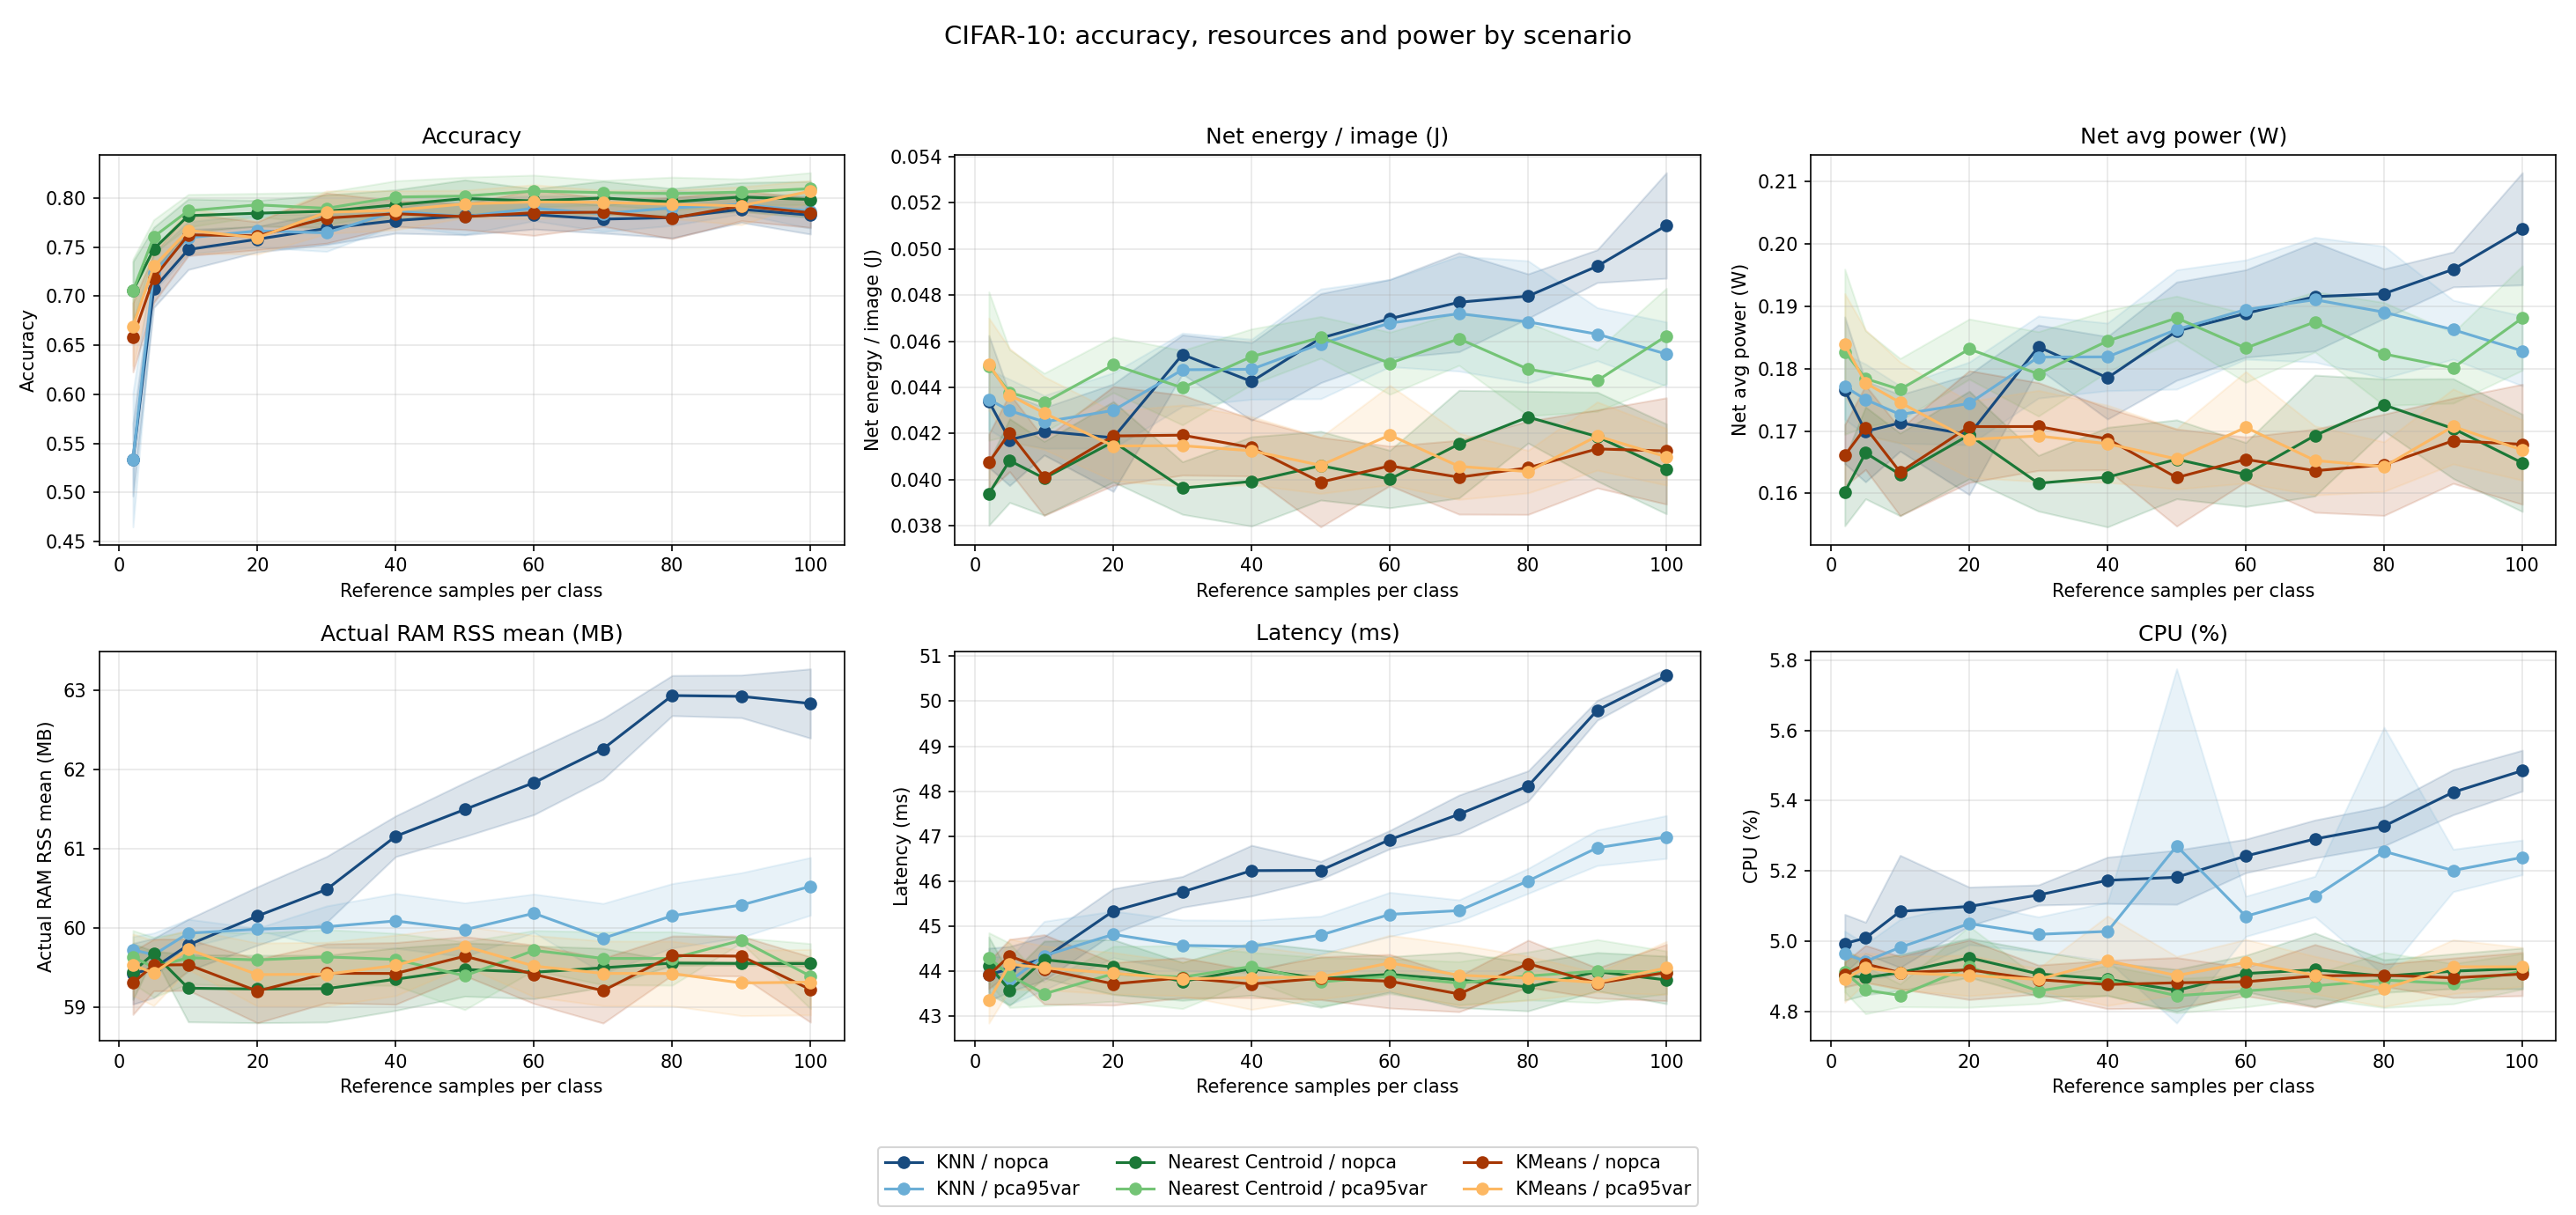
\includegraphics[width=\textwidth]{benchmark/analysis/exports/cifar10/analysis_20260705_193251/figures/cifar10_summary_grid.png}
  \caption{CIFAR-10 benchmark summary for the current export.}
  \Description{Benchmark summary grid showing CIFAR-10 accuracy and resource measurements across classifiers, PCA settings, and reference sample counts.}
  \label{fig:cifar10-summary-grid}
\end{figure*}

\begin{figure*}[t]
  \centering
  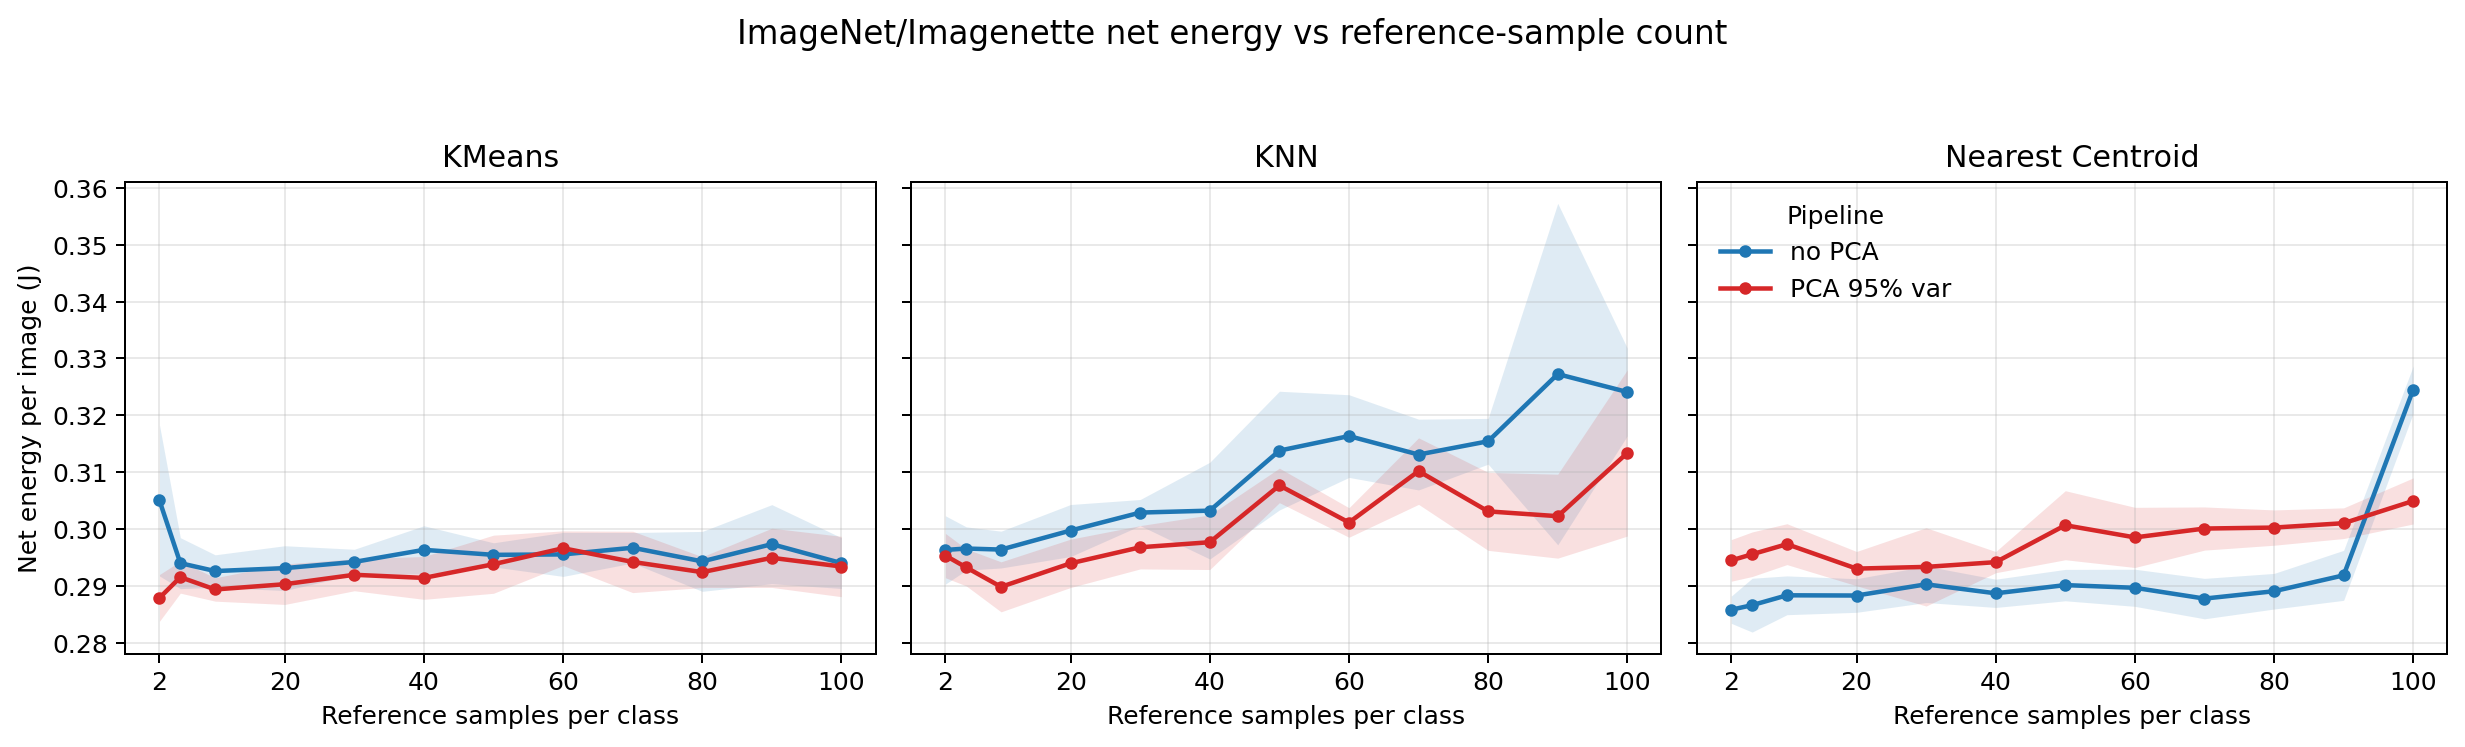
\includegraphics[width=\textwidth]{benchmark/analysis/exports/imagenet/analysis_20260708_140042/figures/imagenet_energy_vs_samples.png}
  \caption{Imagenette net energy per image across reference-sample counts for the corrected export.}
  \Description{Line plots for KMeans, KNN, and Nearest Centroid showing no-PCA and pca95var net energy per image across reference-sample counts. The PCA and no-PCA curves remain close instead of showing a systematic PCA energy penalty.}
  \label{fig:imagenet-energy-samples}
\end{figure*}

\subsection{RQ1: Algorithm Selection}
Table~\ref{tab:best-accuracy} reports the best observed mean accuracy for each classifier and PCA configuration.
For CIFAR-10, the highest observed mean accuracy is 0.8095 for Nearest Centroid with \texttt{pca95var} at 100 samples per class.
KMeans reaches 0.8070 with \texttt{pca95var} at 100 samples per class, while KNN reaches 0.7935 with \texttt{pca95var} at 90 samples per class.
Without PCA, the best CIFAR-10 mean accuracies are 0.8010 for Nearest Centroid, 0.7920 for KMeans, and 0.7885 for KNN.

For Imagenette, KNN has the highest observed mean accuracy with 0.9835 using \texttt{pca95var} at 100 samples per class and 0.9830 without PCA at 100 samples per class.
Nearest Centroid reaches 0.9820 with \texttt{pca95var} at 90 samples per class and 0.9795 without PCA at 100 samples per class.
KMeans reaches 0.9730 with \texttt{pca95var} and 0.9715 without PCA, both at 100 samples per class.

\begin{table*}[t]
  \caption{Best observed mean accuracy per dataset, classifier, and PCA configuration.}
  \label{tab:best-accuracy}
  \centering
  \footnotesize
  \begin{tabular}{@{}lllrrr@{}}
    \toprule
    Dataset & Classifier & PCA & Samples/class & Accuracy mean & 95\% CI \\
    \midrule
    CIFAR-10 & KMeans & nopca & 90 & 0.7920 & 0.0152 \\
    CIFAR-10 & KMeans & pca95var & 100 & 0.8070 & 0.0108 \\
    CIFAR-10 & KNN & nopca & 90 & 0.7885 & 0.0134 \\
    CIFAR-10 & KNN & pca95var & 90 & 0.7935 & 0.0097 \\
    CIFAR-10 & Nearest Centroid & nopca & 90 & 0.8010 & 0.0148 \\
    CIFAR-10 & Nearest Centroid & pca95var & 100 & 0.8095 & 0.0163 \\
    Imagenette & KMeans & nopca & 100 & 0.9715 & 0.0109 \\
    Imagenette & KMeans & pca95var & 100 & 0.9730 & 0.0111 \\
    Imagenette & KNN & nopca & 100 & 0.9830 & 0.0081 \\
    Imagenette & KNN & pca95var & 100 & 0.9835 & 0.0059 \\
    Imagenette & Nearest Centroid & nopca & 100 & 0.9795 & 0.0099 \\
    Imagenette & Nearest Centroid & pca95var & 90 & 0.9820 & 0.0064 \\
    \bottomrule
  \end{tabular}
\end{table*}

The resource summaries show that CIFAR-10 mean net energy per image ranges from 0.0407~J for Nearest Centroid without PCA to 0.0456~J for KNN without PCA.
The corresponding mean latency values range from 43.87~ms for KMeans without PCA to 46.56~ms for KNN without PCA.
For Imagenette without PCA, mean net energy per image ranges from 0.2918~J for Nearest Centroid to 0.3088~J for KNN.
With \texttt{pca95var}, the Imagenette mean net energy per image ranges from 0.2923~J for KMeans to 0.3004~J for KNN.
The corresponding Imagenette PCA net power values are approximately 0.50--0.51~W, comparable to the no-PCA range of approximately 0.51--0.52~W.
Table~\ref{tab:resource-summary} summarizes these resource measurements together with latency and observed RSS memory.

\subsection{RQ2: Reference Sample Sweet Spot}
Table~\ref{tab:sweet-spots} reports the reference-sample knees using two thresholds: the first number of samples per class that reaches at least 95\% of the maximum observed mean accuracy, and the corresponding number for 99\%.
For CIFAR-10 at the 95\% threshold, KMeans reaches the knee at 10 samples per class with and without PCA.
KNN reaches the 95\% knee at 20 samples per class without PCA and at 10 with \texttt{pca95var}.
Nearest Centroid reaches the 95\% knee at 10 samples per class in both PCA settings.

For Imagenette at the 95\% threshold, KMeans and KNN reach the knee at 10 samples per class in both PCA settings.
Nearest Centroid reaches the 95\% knee at 5 samples per class with and without PCA.
At the stricter 99\% threshold, CIFAR-10 knees range from 40 to 100 samples per class, while Imagenette knees range from 10 to 80 samples per class.

\begin{table*}[t]
  \caption{Reference-sample knees at 95\% and 99\% of the maximum observed mean accuracy.}
  \label{tab:sweet-spots}
  \centering
  \footnotesize
  \begin{tabular}{@{}lllrrr@{}}
    \toprule
    Dataset & Classifier & PCA & Max accuracy & 95\% knee & 99\% knee \\
    \midrule
    CIFAR-10 & KMeans & nopca & 0.7920 & 10 & 60 \\
    CIFAR-10 & KMeans & pca95var & 0.8070 & 10 & 100 \\
    CIFAR-10 & KNN & nopca & 0.7885 & 20 & 50 \\
    CIFAR-10 & KNN & pca95var & 0.7935 & 10 & 40 \\
    CIFAR-10 & Nearest Centroid & nopca & 0.8010 & 10 & 40 \\
    CIFAR-10 & Nearest Centroid & pca95var & 0.8095 & 10 & 50 \\
    Imagenette & KMeans & nopca & 0.9715 & 10 & 60 \\
    Imagenette & KMeans & pca95var & 0.9730 & 10 & 80 \\
    Imagenette & KNN & nopca & 0.9830 & 10 & 40 \\
    Imagenette & KNN & pca95var & 0.9835 & 10 & 40 \\
    Imagenette & Nearest Centroid & nopca & 0.9795 & 5 & 10 \\
    Imagenette & Nearest Centroid & pca95var & 0.9820 & 5 & 10 \\
    \bottomrule
  \end{tabular}
\end{table*}

\begin{table*}[t]
  \caption{Resource and energy summary averaged across the full sample-count sweep and seeds. RSS denotes mean observed resident set size; these values summarize global benchmark behavior rather than one selected sweet-spot configuration.}
  \label{tab:resource-summary}
  \centering
  \footnotesize
  \begin{tabular}{@{}lllrrrr@{}}
    \toprule
    Dataset & Classifier & PCA & Net power (W) & Net energy/img (J) & Latency (ms) & RSS (MB) \\
    \midrule
    CIFAR-10 & KMeans & nopca & 0.1669 & 0.0410 & 43.87 & 59.44 \\
    CIFAR-10 & KMeans & pca95var & 0.1705 & 0.0418 & 43.90 & 59.49 \\
    CIFAR-10 & KNN & nopca & 0.1838 & 0.0456 & 46.56 & 61.24 \\
    CIFAR-10 & KNN & pca95var & 0.1825 & 0.0450 & 45.09 & 60.04 \\
    CIFAR-10 & Nearest Centroid & nopca & 0.1659 & 0.0407 & 43.90 & 59.44 \\
    CIFAR-10 & Nearest Centroid & pca95var & 0.1828 & 0.0449 & 43.90 & 59.60 \\
    Imagenette & KMeans & nopca & 0.5190 & 0.2957 & 345.73 & 66.35 \\
    Imagenette & KMeans & pca95var & 0.5039 & 0.2923 & 356.13 & 68.72 \\
    Imagenette & KNN & nopca & 0.5222 & 0.3088 & 367.29 & 79.38 \\
    Imagenette & KNN & pca95var & 0.5089 & 0.3004 & 366.38 & 75.21 \\
    Imagenette & Nearest Centroid & nopca & 0.5130 & 0.2918 & 344.83 & 65.69 \\
    Imagenette & Nearest Centroid & pca95var & 0.5136 & 0.2978 & 355.86 & 68.38 \\
    \bottomrule
  \end{tabular}
\end{table*}

\subsection{RQ3: PCA Influence}
Table~\ref{tab:pca-effect} reports paired PCA effects as \texttt{pca95var} minus \texttt{nopca}.
For CIFAR-10, PCA increases mean accuracy by 0.0088 for KMeans, 0.0060 for KNN, and 0.0066 for Nearest Centroid.
The CIFAR-10 net-energy difference is +0.0009~J per image for KMeans, -0.0007~J per image for KNN, and +0.0042~J per image for Nearest Centroid.

For Imagenette, the paired mean accuracy differences are +0.0017 for KMeans, -0.0020 for KNN, and +0.0014 for Nearest Centroid.
The paired mean net-energy differences are -0.0034~J per image for KMeans, -0.0084~J per image for KNN, and +0.0060~J per image for Nearest Centroid.

\begin{table*}[t]
  \caption{Paired PCA effect by dataset, classifier, and metric. Delta is \texttt{pca95var} minus \texttt{nopca}.}
  \label{tab:pca-effect}
  \centering
  \footnotesize
  \begin{tabular}{@{}lllrrrr@{}}
    \toprule
    Dataset & Classifier & Metric & Pairs & PCA mean & no-PCA mean & Delta \\
    \midrule
    CIFAR-10 & KMeans & Accuracy & 120 & 0.7731 & 0.7643 & +0.0088 \\
    CIFAR-10 & KMeans & Net energy/img (J) & 120 & 0.0418 & 0.0410 & +0.0009 \\
    CIFAR-10 & KNN & Accuracy & 120 & 0.7549 & 0.7489 & +0.0060 \\
    CIFAR-10 & KNN & Net energy/img (J) & 118 & 0.0450 & 0.0457 & -0.0007 \\
    CIFAR-10 & Nearest Centroid & Accuracy & 120 & 0.7893 & 0.7826 & +0.0066 \\
    CIFAR-10 & Nearest Centroid & Net energy/img (J) & 120 & 0.0449 & 0.0407 & +0.0042 \\
    Imagenette & KMeans & Accuracy & 120 & 0.9398 & 0.9381 & +0.0017 \\
    Imagenette & KMeans & Net energy/img (J) & 120 & 0.2923 & 0.2957 & -0.0034 \\
    Imagenette & KNN & Accuracy & 120 & 0.9455 & 0.9475 & -0.0020 \\
    Imagenette & KNN & Net energy/img (J) & 120 & 0.3004 & 0.3088 & -0.0084 \\
    Imagenette & Nearest Centroid & Accuracy & 120 & 0.9716 & 0.9702 & +0.0014 \\
    Imagenette & Nearest Centroid & Net energy/img (J) & 119 & 0.2978 & 0.2918 & +0.0060 \\
    \bottomrule
  \end{tabular}
\end{table*}

\section{Discussion}
The results show that the most suitable distance-based architecture depends on the dataset and on whether the target prioritizes maximum accuracy or resource-efficient operation.
Across both datasets, only a small number of stored reference samples per class is needed to reach most of the attainable accuracy.
The effect of PCA is dataset-dependent: it improves CIFAR-10 accuracy slightly, and on Imagenette its energy changes remain small while accuracy changes only marginally.

\subsection{Answering the Research Questions}
\paragraph{RQ1 -- Algorithm Selection.}
The goal of RQ1 was to determine how the choice of distance-based classifier affects the trade-off between accuracy and efficiency in the TinyMLOps framework.
On CIFAR-10, Nearest Centroid achieved the highest observed mean accuracy with 0.8095 using \texttt{pca95var}, while also remaining close to KMeans in latency and memory usage.
On Imagenette, KNN achieved the highest observed mean accuracy with 0.9835 using \texttt{pca95var}, while its no-PCA variant already reached 0.9830 with comparable energy consumption.
Overall, Nearest Centroid is a strong compact candidate, whereas KNN is most attractive when the highest Imagenette accuracy is prioritized and the additional reference-store cost is acceptable.

\paragraph{RQ2 -- Reference Sample Sweet Spot.}
The goal of RQ2 was to identify how many stored reference samples per class are needed before additional samples provide only limited accuracy gains.
For the 95\% threshold, most configurations reach their knee at 10 samples per class; the exceptions are CIFAR-10 KNN without PCA at 20 samples per class and Imagenette Nearest Centroid at 5 samples per class.
At the stricter 99\% threshold, CIFAR-10 requires between 40 and 100 samples per class, while Imagenette requires between 10 and 80 samples per class depending on classifier and PCA setting.
Thus, 10 samples per class is a practical low-cost operating point for most configurations, while 40 to 60 samples per class are more appropriate when near-maximum accuracy is required.

\paragraph{RQ3 -- PCA Influence.}
The goal of RQ3 was to evaluate whether PCA improves the accuracy-efficiency trade-off for the evaluated distance-based classifiers.
On CIFAR-10, \texttt{pca95var} improves mean accuracy for all three classifiers by 0.0060 to 0.0088, with only small energy changes for KMeans and KNN but a larger energy increase for Nearest Centroid.
On Imagenette, PCA changes mean accuracy only marginally, ranging from -0.0020 for KNN to +0.0017 for KMeans, while paired net-energy differences remain close to zero between -0.0084 and +0.0060~J per image.
Therefore, PCA is useful for CIFAR-10 when a small accuracy gain is desired and is attractive on Imagenette when dimensionality reduction is valuable and small energy changes are acceptable.

\subsection{Improvement Potentials}
The first improvement potential concerns the PCA implementation for high-dimensional Imagenette features.
PCA reduces the feature dimensionality from 1280 to 608 with only small measured energy changes in the corrected Imagenette measurements.
Future work should still profile the PCA transformation separately from the classifier step and evaluate whether precomputed or quantized projection matrices further improve deployment efficiency.

The second improvement potential is the selection of benchmark operating points.
The current sweep covers a broad range from 2 to 100 samples per class, but the observed knees indicate that the most informative region lies between 5 and 60 samples per class for most configurations.
Future experiments should use a denser sweep in this region and fewer runs at clearly saturated sample counts, which would reduce benchmark time while improving resolution around the actual sweet spot.

The third improvement potential is the treatment of use-case constraints.
The current analysis reports accuracy, latency, memory, CPU, and energy, but it does not yet convert these metrics into a single deployment decision rule.
Future versions of the framework should allow users to specify constraints such as maximum memory, maximum energy per image, or minimum accuracy, and then automatically rank feasible configurations.

The fourth improvement potential is broader external validation.
The current benchmark uses CIFAR-10 and Imagenette with ten seeds and a median of 200 test images per run.
Additional datasets, different numbers of classes, and task-specific embedded use cases would make it easier to determine whether the observed sample-count knees and PCA behavior generalize beyond the evaluated image-classification scenarios.

\subsection{Threat to Validity}
\paragraph{Internal validity.}
Internal validity may be affected by measurement noise on the target device.
Although the experiments were repeated across ten seeds and power measurements were collected with an external power supply, background activity on the Raspberry Pi Zero 2W, thermal effects, and operating-system scheduling can still influence latency, CPU, RSS memory, and energy measurements.
BLAS/OpenMP execution was pinned to one thread for clean single-threaded energy measurement.
The study reduces this risk by aggregating results across seeds and by reporting confidence intervals, but it cannot fully eliminate device-level noise.
Another internal threat is that PCA is measured as part of the deployed inference pipeline; therefore, the reported PCA effect includes both dimensionality reduction and classification effects rather than isolating the classifier alone.

\paragraph{Construct validity.}
Construct validity concerns whether the collected metrics adequately represent the intended accuracy-efficiency trade-off.
Accuracy, latency, CPU usage, RSS memory, analytical classifier state size, and net energy per image cover the main deployment-relevant dimensions, but they do not capture all aspects of an embedded system.
For example, flash usage, long-term battery behavior, thermal throttling over extended operation, and retraining cost after deployment are not represented as separate optimization targets.
The chosen 95\% and 99\% accuracy knees provide clear operational definitions of a sweet spot, but different applications may define an acceptable accuracy loss differently.

\paragraph{Conclusion validity.}
Conclusion validity may be affected by the finite number of repeated runs and by the selected benchmark grid.
Each configuration is evaluated across ten seeds, which supports comparative analysis, but small differences such as the Imagenette PCA accuracy changes remain close to the scale of experimental variation.
The study reports paired PCA comparisons where matched pairs exist, yet it does not claim that every small numeric difference is practically relevant.
The sample-count sweep also uses discrete values between 2 and 100 samples per class, so the exact sweet spot may lie between two evaluated sample counts.

\paragraph{External validity.}
External validity is limited by the evaluated hardware, datasets, and task structure.
The experiments use a Raspberry Pi Zero 2W and image-classification benchmarks based on CIFAR-10 and Imagenette; the resulting trade-offs may differ on microcontrollers, accelerators, or sensors with different feature-extraction pipelines.
A relevant threat to external validity is that the number of classes is not varied in this study.
Therefore, the final configuration recommendation cannot be transferred directly to binary use cases such as obstacle detection, because the trade-off between accuracy and efficiency may differ in such settings.
Additional datasets, class counts, hardware platforms, and real deployment workloads are needed before generalizing the observed sweet spots to all TinyML use cases.

\section{Conclusion}
This work evaluated distance-based architectures for on-device learning in the TinyMLOps framework.
The study compared KMeans, KNN, and Nearest Centroid on CIFAR-10 and Imagenette using both no-PCA and \texttt{pca95var} variants, a reference-sample sweep from 2 to 100 samples per class, and ten seeds per configuration.
The evaluation considered prediction accuracy together with resource-related measurements such as latency, CPU usage, memory consumption, and net energy per image.

The results show that a small number of reference samples is sufficient to reach most of the attainable accuracy.
At the 95\% accuracy threshold, most configurations reach their knee at 10 samples per class, with CIFAR-10 KNN without PCA requiring 20 samples per class and Imagenette Nearest Centroid reaching the knee already at 5 samples per class.
Nearest Centroid provides a strong compact configuration on CIFAR-10, while KNN achieves the highest observed Imagenette accuracy.
PCA improves CIFAR-10 accuracy slightly and is attractive on Imagenette when dimensionality reduction is valuable, with measured energy changes remaining small.

Future work should continue to profile the PCA projection separately, especially for high-dimensional Imagenette features.
The benchmark should also use denser sample-count sweeps around the observed knees and integrate deployment constraints such as maximum energy, memory, or latency into the configuration-selection process.
Finally, the results should be validated on additional datasets, different class counts, and further embedded hardware platforms before generalizing the recommended sweet spots to broader TinyML use cases.

%%
%% The acknowledgments section is defined using the "acks" environment
%% (and NOT an unnumbered section). This ensures the proper
%% identification of the section in the article metadata, and the
%% consistent spelling of the heading.




%%
%% The next two lines define the bibliography style to be used, and
%% the bibliography file.
\bibliographystyle{ACM-Reference-Format}
\bibliography{sample-base}


%%
%% If your work has an appendix, this is the place to put it.


\end{document}
\endinput
%%
%% End of file `sample-sigconf-authordraft.tex'.
